\documentclass[./AutomatedMK.tex]{subfiles}


\begin{document}
% ============================================================================================================
\section{Discussion}\label{sec:discussion2}

	Figures \ref{fig:KNNR}  and \ref{fig:RFR} and Tables \ref{tab:KNN} and \ref{tab:RF} show that classification using KNN has essentially the same accuracy as RF. These Figures and Tables demonstrate that using KNN and RF along side Algorithm \hyperlink{alg:FS}{1} for feature selection are viable options for the automated classification of stellar spectra because of the high accuracy achieved.

Figure \ref{fig:KNNR} and Table \ref{tab:KNN} demonstrate that using three neighbors for KNN classification performs the best. Figure \ref{fig:RFR} and Table \ref{tab:RF} shows that changing the number of trees used in RF does not significantly change the classification accuracy. Figures \ref{fig:KNNR}  and \ref{fig:RFR} show that Oversampling balancing performs best. However, Tables \ref{tab:KNN} and \ref{tab:RF} shows that Oversampling balancing (2,657,466 samples) only outperforms Hybrid balancing (957,398 samples) by roughly one percent. Figures \ref{fig:KNNPRF} and \ref{fig:RFPRF} and Tables \ref{tab:PRFKNN} and \ref{tab:PRFRF} show that the Precision, Recall, and F1 Score are all roughly the same for each experiment. 

Tables \ref{tab:KNNT} and \ref{tab:RFT} show the execution times for each experiment. These tables show that KNN performs much faster than RF. KNN has a faster train time than RF. but RF has a faster test time than KNN. For both KNN and RF, feature selection takes the same amount of time, which is expected since they both use the same feature selection.
	
This approach takes considerably fewer steps than the one in \citeauthor{Bolton} and produces excellent results. The execution times and the obtained accuracy demonstrate that, for a real application of this work, the automated classification of redshifted stellar spectra into a complete MK classification using a single classifier not only achieves a high accuracy but is also fast.

As described above in Section \ref{sec:Approach_B}, these experiments deal with data collected by a real astronomical survey. As such, when an astronomical survey points their telescopes into the sky, they get the samples (classes) that they get. These experiments deal with a subset of all possible class combinations. It is important to note that not all possible class combinations (O, B, A, F, G, K, and M with sub - classes of 0 - 9 combined with I, II, III, IV, V, VII) are common or even found in nature. Therefore, even though this approach yielded great results, there cannot be a claim that this approach will guarantee work for all stellar classes. There is, however, some theoretical validity to this approach. 

We have to recall that the spectral classes are based on absorption lines and the luminosity classes are based on the widths of those absorption lines \citep{Gray}. Also, according to Section \ref{sec:Approach_B}, the shape, intensity, and width of the absorption lines are preserved (seen in Figs. \ref{fig:B}, \ref{fig:A},  \ref{fig:F}, \ref{fig:G}, \ref{fig:K}, and \ref{fig:M}). Referencing Fig. \ref{fig:O}, O type stars also contain the H$_\delta$ absorption line. This strengthens the theoretical validity because the missing spectral major class would also be represented using this approach. 

As stated in Section \ref{sec:Approach_B}, the widths of the absorption lines are also preserved. This provides strength to the theoretical validity because every spectral major class would have at least one absorption line preserved and in turn, the widths preserved. This means that this approach should work with the missing spectral and luminosity class combinations, assuming the model was retrained. 

        \begin{figure}
            \centering
             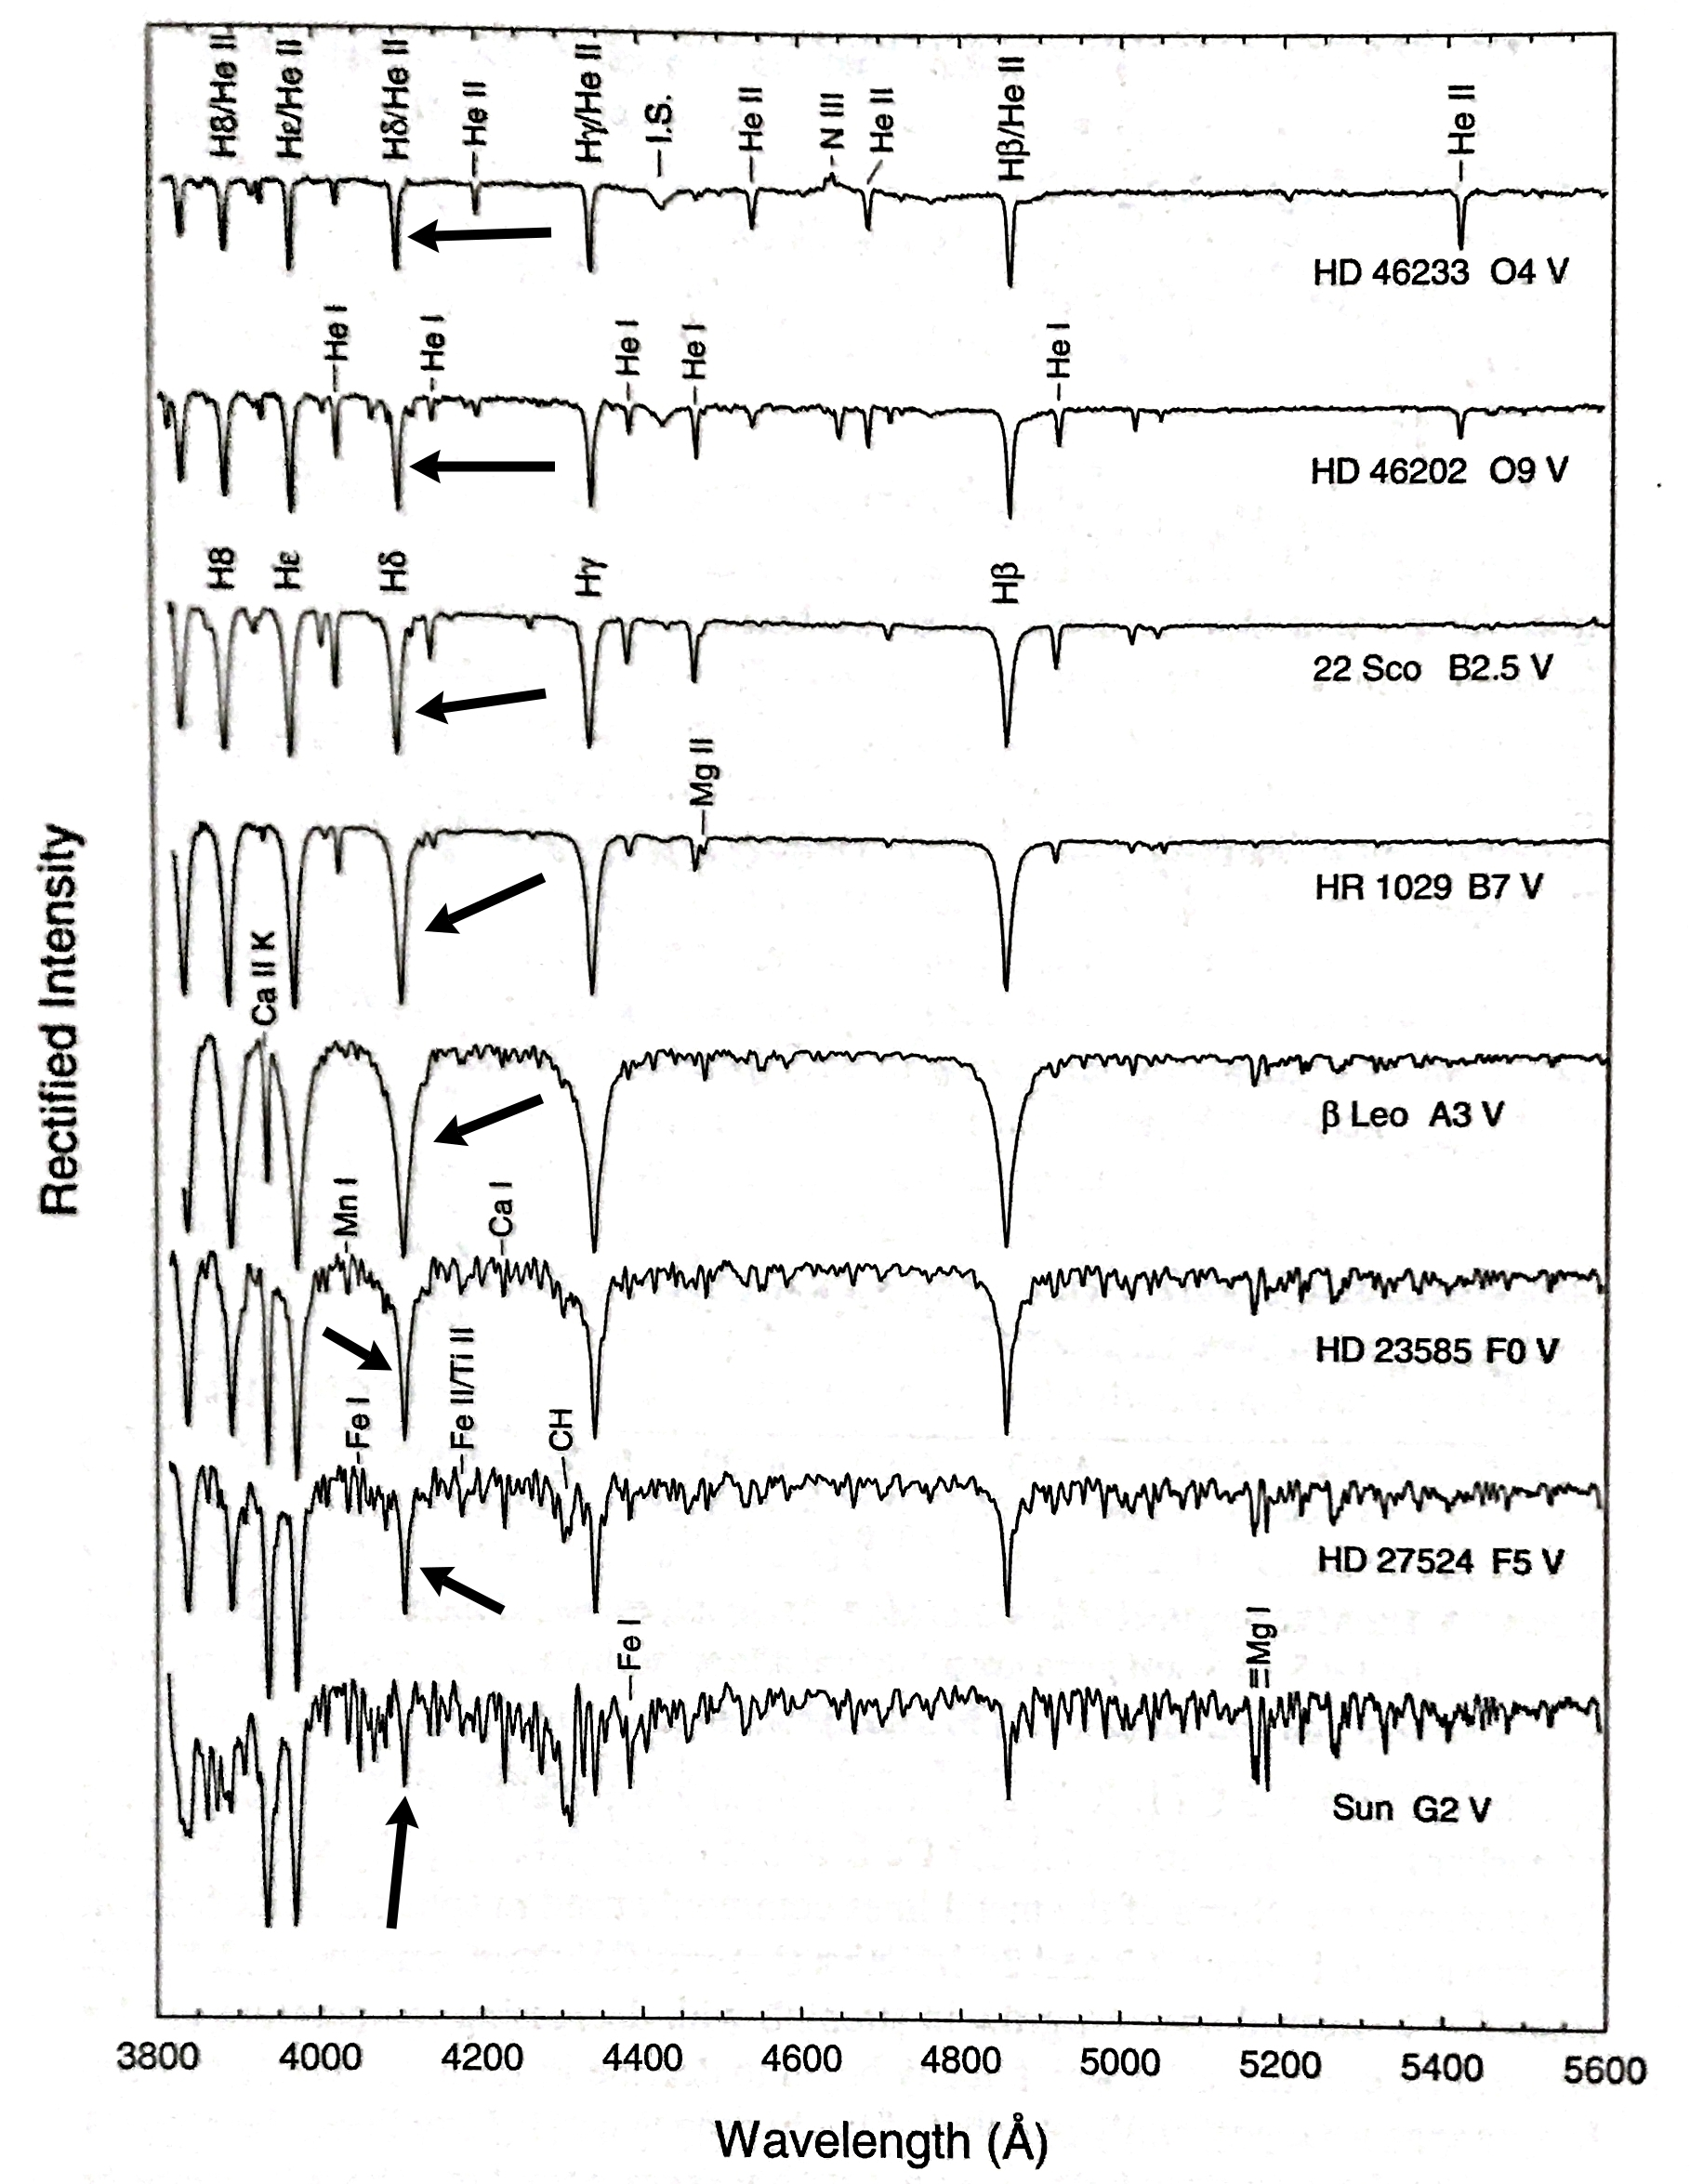
\includegraphics[width=.5\linewidth]{figures/OStar.jpeg}
            \caption{Sample of continuum normalized spectra from O - G type stars, \citep{Gray}. The arrows point to the H$_\delta$ absorption line}
            \label{fig:O}
        \end{figure}

\end{document}